\subsection{Example}\label{sec:sample-example}

We have observed how the set-based approach to solving inverse problems can lead to errors in approximating measures, particularly around the boundaries of the solution set.
The sample-based approach that we summarized above does not rely on Voronoi-cell approximations of contour events, instead assigning probability to random samples drawn from an initial density.

We demonstrate that for estimating a uniform density over a subset of the initial parameter space, the sample-based approach is able to more accurately approximate it at a given sample size.
The reason for this is that the approach has a different source of error, involving estimating to push forward of the initial density.
We are interested in studying how our ability to estimate a uniform density is impacted by the number of samples drawn from the initial density.

We solve the same problem as before but use a uniform initial density in place of a uniform ansatz.
We sample 100, 1,000 and 10,000 samples from the initial density and use Gaussian kernel density estimation to approximate the denominator in Eq [TK - eq], and show the resulting updated densities in Figure.

Observe that the support of the updated density matches the solution of the previous inverse problem but is much more accurately approximated. Gone are the jagged edges that we saw before. The relative probability is assigned within the support are also more similar to one another, something we demonstrate in the next Figure, which shows conditional densities along the unit directions through the center of the domain.

We are interested in studying how our ability to estimate a uniform density is impacted by the number of samples drawn from the initial density.
We form an inverse problem with the identity map an standard uniform initial densities, with observed densities being uniform over $[0.4, 0.6]^2$, representing a hundred-fold reduction in uncertainty when the problem is solved

We solve the same problem as before but use a uniform initial density in place of a uniform ansatz.
We sample $N=100$, $1,000$ and $10,000$ samples from the initial density and use Gaussian kernel density estimation to approximate the denominator in Eq [TK - eq], and show the resulting updated densities in Figure~\ref{fig:ex:identity_sampling_approx}.

Observe that the support of the updated density matches the solution of the previous inverse problem but is much more accurately approximated.
Gone are the jagged edges that we saw before, replaced by clean squares.
The relative probability is assigned within the support are also more similar to one another, something we demonstrate in Figure~\ref{fig:identity_sampling_conditionals}, which shows conditional densities along the unit directions through the center of the domain.

\begin{figure}[ht]
\begin{minipage}{.975\textwidth}
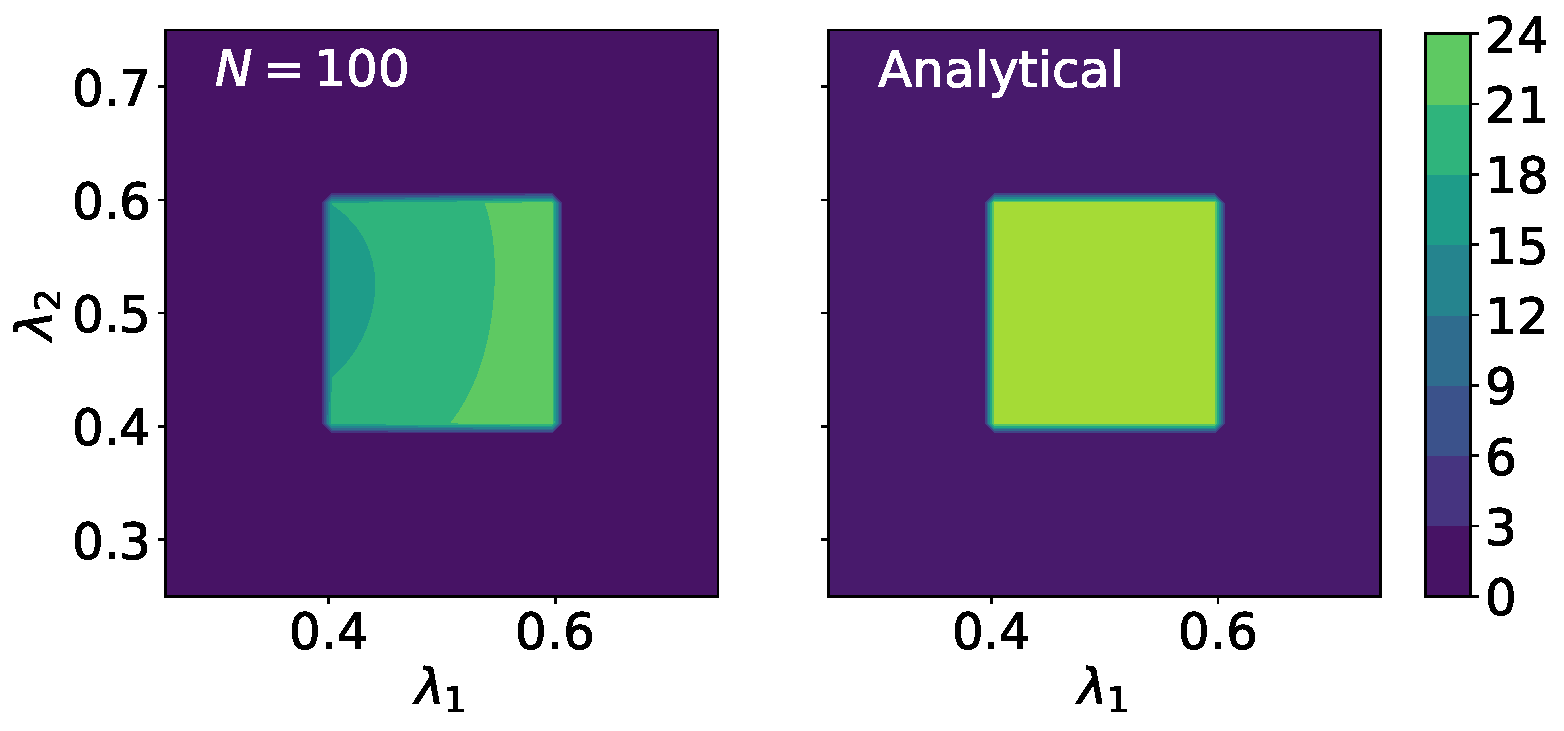
\includegraphics[width=\linewidth]{./examples/identity/samp/N100_N100-vs-Analytical_N100.pdf}
\end{minipage}
\caption{
(Left): $\nsamps=100$ were used to construct the predicted distribution $\predicted$.
(Right): By specifying an analytical $\predicted$, the effect of using $\nsamps$ to approximate a pushforward distribution disappears. The problem can be fully specified in BET without any random sampling.
}
\label{fig:ex:identity_sampling_exact}
\end{figure}

\begin{figure}[ht]
\begin{minipage}{.975\textwidth}
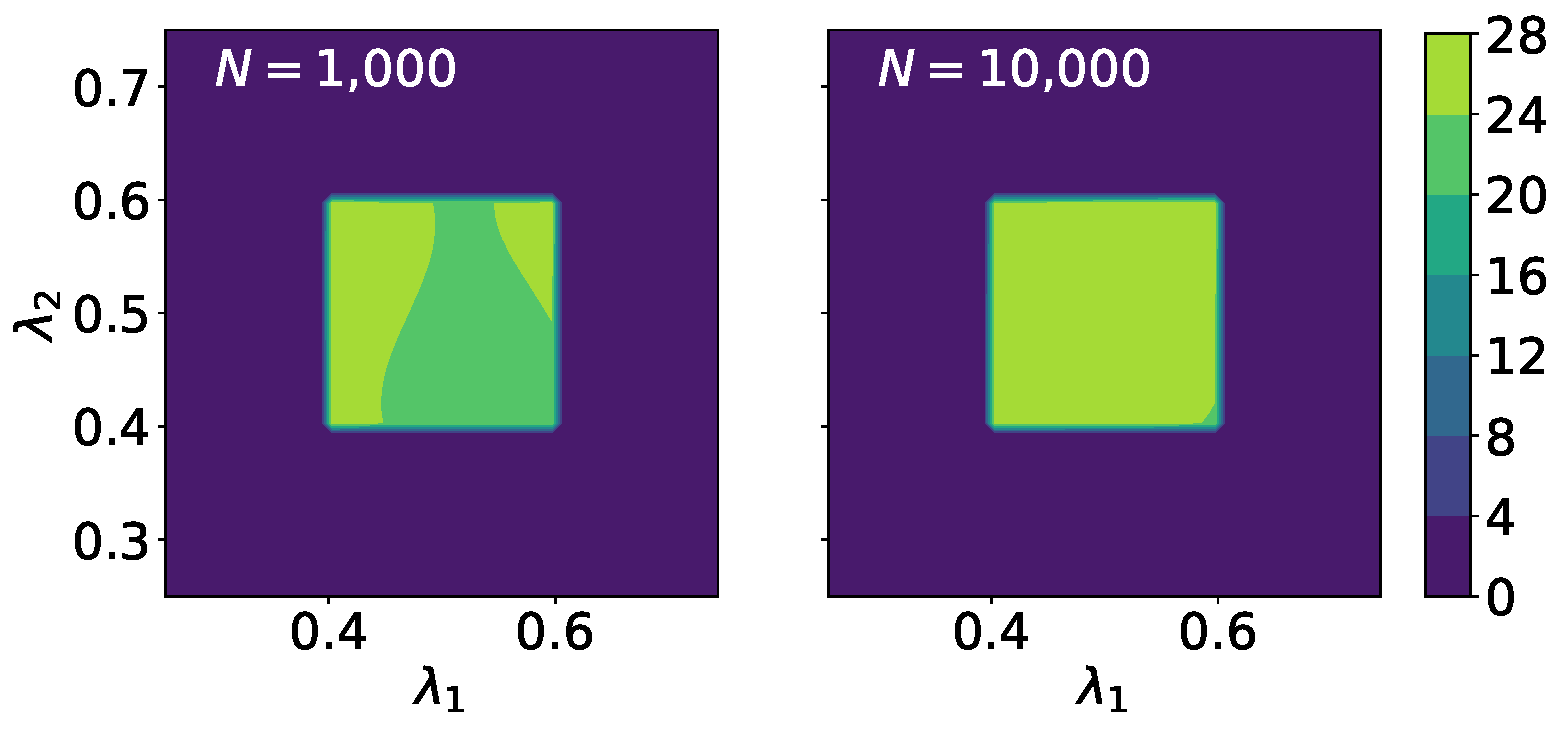
\includegraphics[width=\linewidth]{./examples/identity/samp/N1-000_N1000-vs-N10-000_N10000.pdf}
\end{minipage}
\caption{
$\nsamps=1,000$ (left) and $\nsamps=10,000$(right) were used to construct the predicted distribution $\predicted$.
There is no signficant error in estimating the support of the distribution, only the density approximation itself.
}
\label{fig:ex:identity_sampling_approx}
\end{figure}

\begin{figure}[ht]
\centering
% N = 1E2
\begin{minipage}{.975\textwidth}
		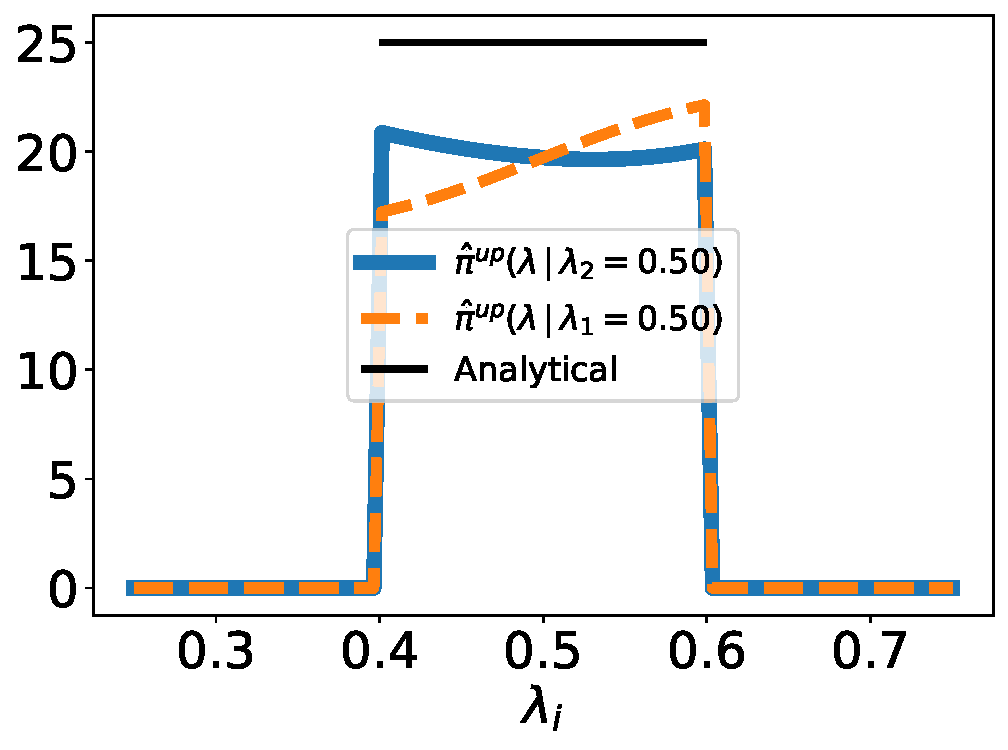
\includegraphics[width=0.5\linewidth]{./examples/identity/samp/identity_1d_conditionals_50E-2_N100_approx.pdf}
    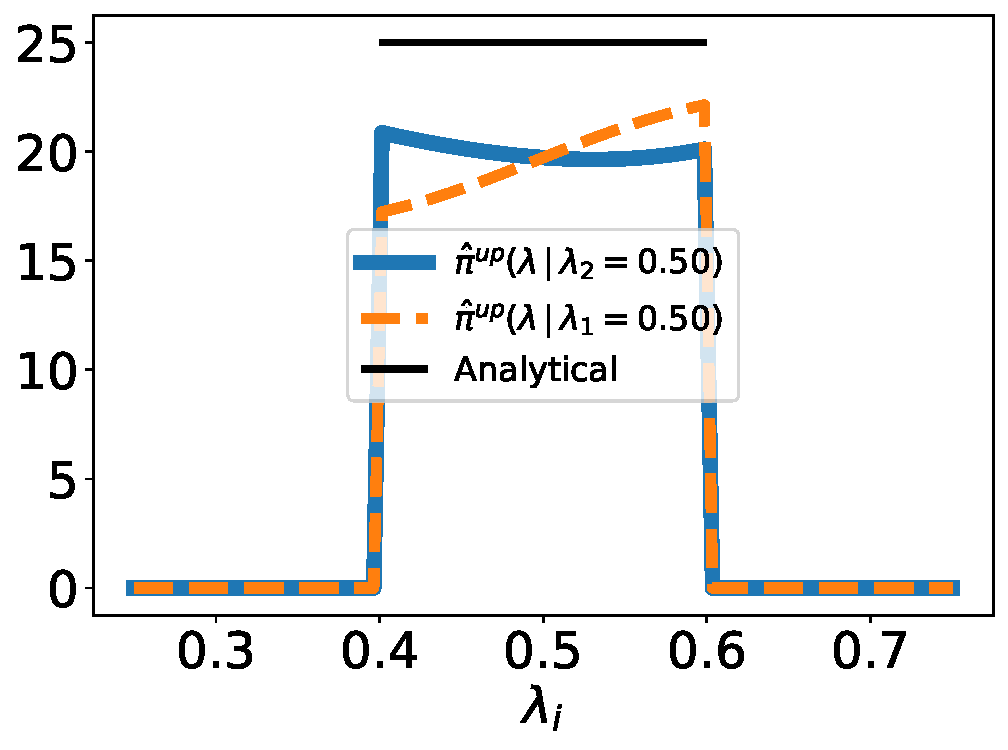
\includegraphics[width=0.5\linewidth]{./examples/identity/samp/identity_1d_conditionals_50E-2_N100_approx.pdf}
\end{minipage}
% N = 1E3
\begin{minipage}{.975\textwidth}
		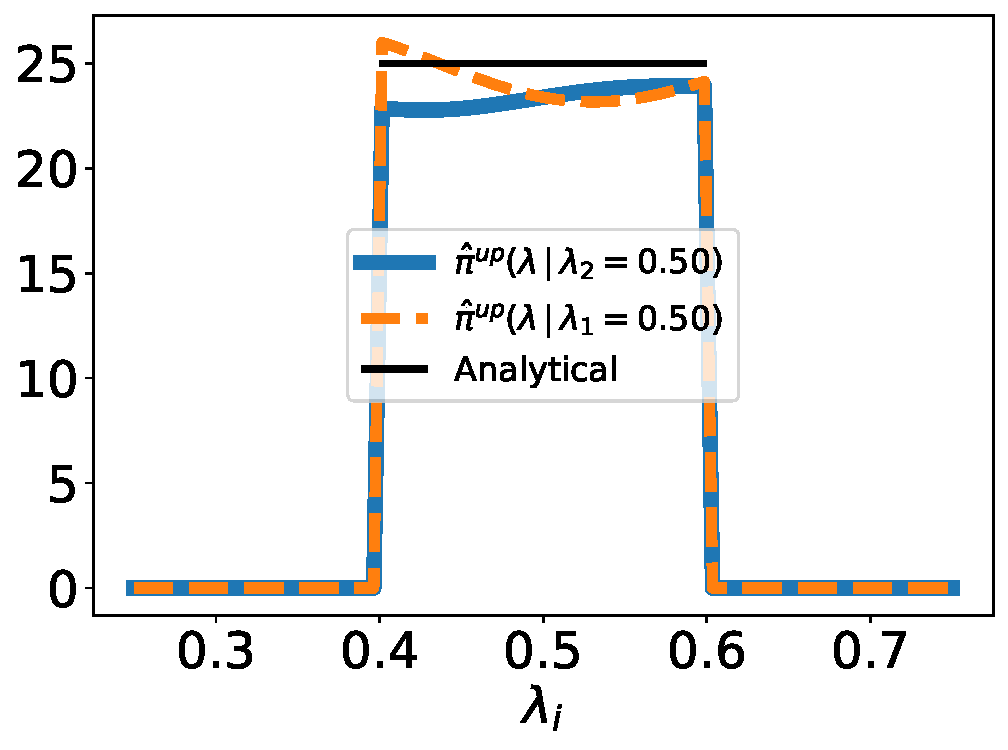
\includegraphics[width=0.5\linewidth]{./examples/identity/samp/identity_1d_conditionals_50E-2_N1000_approx.pdf}
		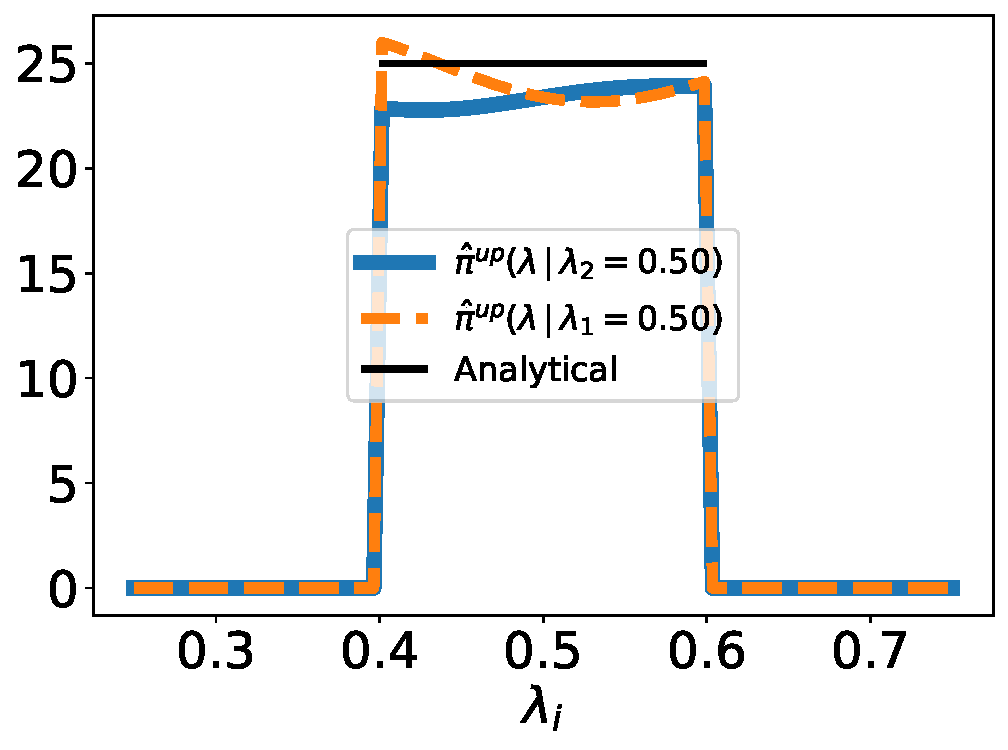
\includegraphics[width=0.5\linewidth]{./examples/identity/samp/identity_1d_conditionals_50E-2_N1000_approx.pdf}
\end{minipage}
% N = 1E4
\begin{minipage}{.975\textwidth}
		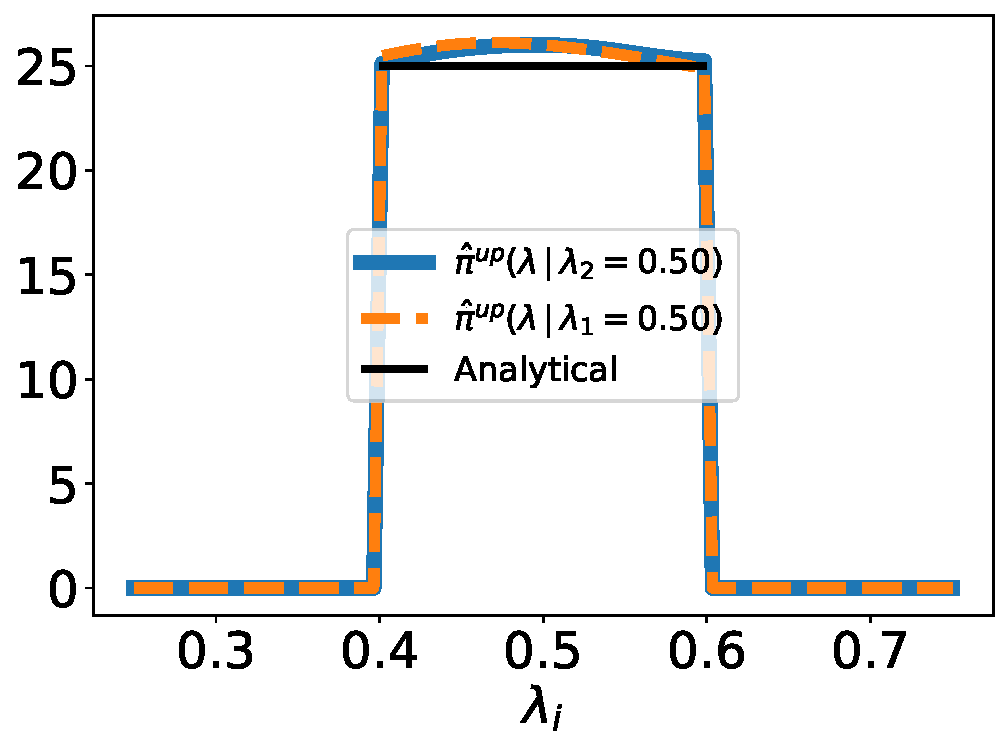
\includegraphics[width=0.5\linewidth]{./examples/identity/samp/identity_1d_conditionals_50E-2_N10000_approx.pdf}
		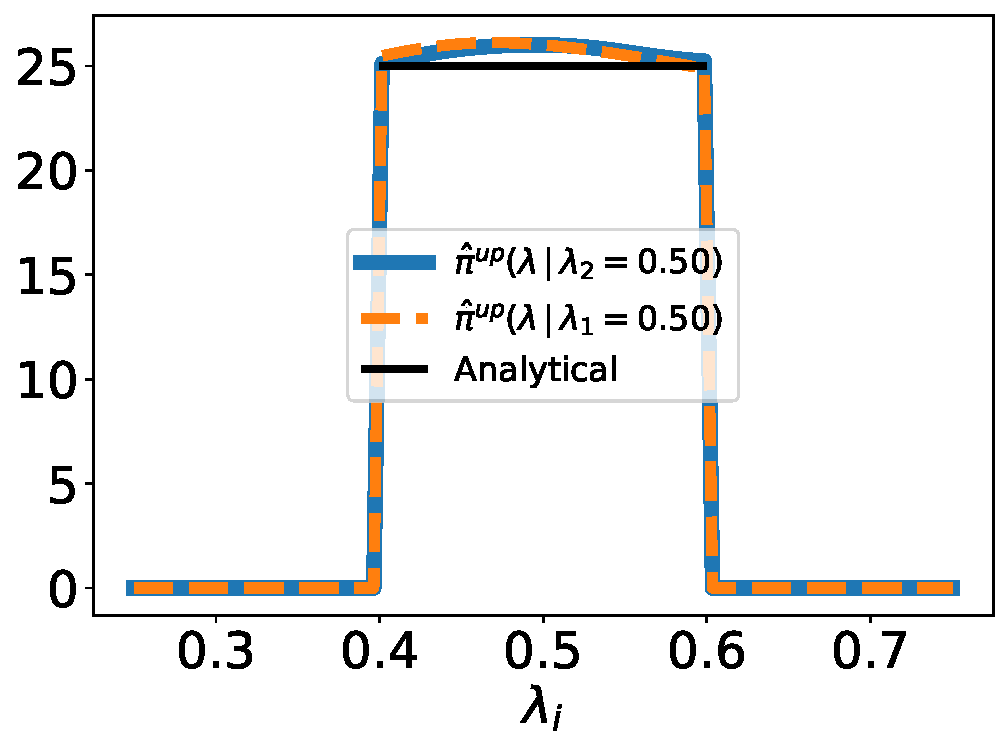
\includegraphics[width=0.5\linewidth]{./examples/identity/samp/identity_1d_conditionals_50E-2_N10000_approx.pdf}
\end{minipage}
\caption{
(Left): $\param_1=0.5$ conditional.
(Right): $\param_2=0.5$ conditional.
(Top to Bottom): Conditional for $\updated$ solutions for  $\nsamps=1E2, 1E3, \text{and} 1E4$ random samples.
}
\label{fig:identity_sampling_conditionals}
\end{figure}
\FloatBarrier

Qualitatively speaking we find that the estimate of the density improve as more samples are used, but at all sample sizes, the support of the density is correctly identified, which we can see by the sharp lines in Fig~\ref{fig:identity_sampling_conditionals} and \ref{fig:ex:identity_sampling_approx}.

The sample-based method trades one source of accuracy for another.
When estimating boundaries of a set which represents an equivalent class of solutions is important, the sample best method provides a compelling alternative to be set based method.

However, we know that this is not without its pitfalls, as density estimation in high dimensions can become prohibitively prone to error.
